\section{Regression}

\section{1D Convolutional Neural Network}

\subsection{Convolution}
\begin{figure}
    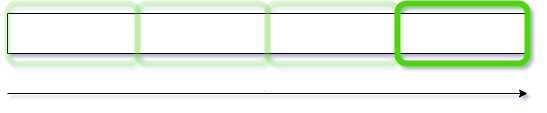
\includegraphics[height=2.5cm]{img/feature_detector.png}
    \caption{Feature Detector / Filter "sliding" over input data}
    \label{figure:feature_detector}
\end{figure}

The main ingredient in a CNN is the \textit{convolutional} layer. It is responsible for, as you may have guessed, the convolution.
It consists of a number of \textit{filters} \ref{figure:feature_detector}, which are the sliding windows that go through the input data. 
They are also called \textit{feature detectors}, and using 100 of them means that the layer can detect 100 features. 
The size of a filter is called \textit{kernel size}. The output of convolutional layer is a matrix with one column for each filter, and one row for each step
in the convolution. How many steps there are, is given by the length of the input data (also called \textit{height}) minus the kernel size plus 1.


\subsection{Creating the Model}
Following the tutorial on 1D CNNs \cite{1d_cnn}, we came up with this model \ref{code:1d_conv_net}. 
We used most of the same parameters, but we also had to tweak some of them to make the model work on our dataset.

To make a convolutional neural network, you need some \textit{convolutional} and \textit{pooling} layers.
Which layers you add in between and the ordering of them, together with the parameters you pass to the layers, 
is what makes the model perform differently. This, of course, requires your input data to be well structured.

\begin{itemize}
  \item We start by defining a \textbf{Sequential} model. This is an easy to understand and readable way of defining a model. 
        Alternatively we could use a \textbf{functional} model, which gives more control of inputs and outputs of the layers.
        A \textbf{functional} model would be useful if we wanted to debug and optimize each layer within the model.
  \item \textbf{Reshape}: In the first layer we need to reshape the input data so that it becomes an $X$ by 1 matrix, where $X$ is the length of each segment.
        The reason for this reshape step is because the next layer (\textbf{Conv1D}) requires the input to contain (\textit{batch, steps, channels}). 
        \textit{Batch} will be set to \textbf{None}, \textit{steps} will be the segments, and \textit{channels} will be $1$ 
        (because we only have one measurement value for each minute).
  \item \textbf{Conv1D}: This is the first \textit{convolutional} layer, where the required parameters are how many \textit{filters} 
        you want, and how big the \textit{kernel} should be. As in the tutorial, we will also start by using 100 filters and a kernel size of 10. 
        Having less or more might impact the performance, which we will experiment on later.
        There are many different parameters that you can use on a layer like this, for example \textit{padding} and \textit{strides},
        but using the default values is good for now. This is also something that we can experiment with later.
        However using the default parameters, the output of this layer will be a $(X-10+1) \times 100$ matrix, 
        and $X$ is the length of each segment here as well.
  \item \textbf{Conv1D}: The second convolutional layer will look exactly like the first one, and the output will be a $(X-10+1-10+1) \times 100$ matrix. 
  \item \textbf{MaxPooling1D}: Pooling is important in a convolutional neural network to reduce complexity \cite{1d_cnn}. 
        The basic idea of \textit{max pooling} is to reduce to only the maximum value for each \textit{window} of size $N \times N$. We are using 2 as 
        window size ($N$), resulting in matrix that is half the size of the input: $ \frac{X-10+1-10+1}{2} \times 100$. 
        Pooling may also help reduce \textit{overfitting}.
  \item \textbf{Conv1D}: Two more convolutional layers are added, and after these the input to the next layer will be a matrix of size
        $ \left( \frac{X-10+1-10+1}{2}-10+1-10+1 \right) \times 160 $.
  \item \textbf{GlobalAveragePooling1D}: This is another pooling layer, and this one takes the average of weights within the network instead of the maximum.
        After doing this, the matrix will be of size $ 1 \times 160 $.
  %\item \textbf{Dropout}: Dropout
  \item \textbf{Dense}: The final layer in the model is a dense layer (fully connected) which reduces the matrix from $160$ values to $2$ with the
        activation function \textbf{softmax}. Then output (a $1$ in one of the two neurons), is mapped to the corresponding label (bipolar/not).
        
\end{itemize}

\subsection{Creating Input Data}
\begin{table}
  \begin{center}
    \begin{tabular}{| l | l |}
      \hline
      \textbf{Not bipolar} & \textbf{Bipolar}  \\ \hline
      0                    &  1                \\ \hline
      1                    &  0                \\ \hline
      0                    &  1                \\ \hline
      1                    &  0                \\ \hline
      1                    &  0                \\ \hline
      0                    &  1                \\ \hline
      0                    &  1                \\ \hline
      1                    &  0                \\ \hline
    \end{tabular}
    \caption{Categorical Labels}
    \label{table:categorical_labels}
  \end{center}
\end{table}

One function (\textit{create\_segments\_and\_labels()} \ref{code:reading_dataset}) is responsible of creating the data that is sent into the neural network. 
It does the following:

\begin{itemize}
  \item First we read the \textit{global} dataset, where we find each participant and whether they are bipolar or not. As there is no \textit{afftype} value
        for non-bipolar participants, we simply set this to 0. This is fine because the other possible values are 1, 2 and 3.
  \item Then we iterate over all participant activity data files:
  \begin{itemize}
    \item Append a \textbf{segment} that is 60 minutes long to the list of segments (using default parameters in the
          \textit{create\_segments\_and\_labels} function \ref{code:reading_dataset}).
    \item Append a 1 if the participant is bipolar, or a 0 if not to the list of labels.
    \item Skip to the next hour, and repeat until we have added all segments.
  \end{itemize}
  \item Make the list of labels into a \textit{categorical} 2D matrix \ref{table:categorical_labels} with a \textbf{1} in only one of the columns,
        instead of a single-dimensional list.
        This is needed for the \textbf{softmax} activation function, which we will describe later.
  \item Also we need the list of segments to be restructured. We do this with the \textbf{reshape} function, 
        and after this the data is ready to be passed into the neural network.
\end{itemize}

\noindent One last step is done before we can start training the model. We need to split the data in two parts; training and test data. This way we can calculate 
the performance of the model after training has finished. The function \textbf{train\_test\_split} from the \textit{sklearn} package is useful here, 
where you input the segments and labels, plus how large you want the training and test sets to be (number between 0 and 1, which determines the size of the 
test partition). The function also randomizes the data, so that the model won't accidentally learn something that is correct for two segments in a row that 
also happen to be chronological.

\section{Optimizing the model}

Ideas: 
\begin{itemize}
    \item Increase segment length, 8 hours is best so far
    \item Tweak other parameters
    \item Switch to functional model, see how well each layer is performing
\end{itemize}

\newpage

\section{Source Code}
\subsection{Create Input Data}
\begin{code}
  \caption{Read Dataset, Create Input Data}
  \label{code:reading_dataset}
  
  \begin{minted}[linenos]{python}
  def create_segments_and_labels(segment_length, output_classes=2, step=60):
    scores = pd.read_csv('scores.csv')
    scores['afftype'].fillna(0, inplace=True)
    
    segments = []
    labels = []

    for person in scores['number']:
      p = scores[scores['number'] == person]
      df_activity = pd.read_csv(f'{person}.csv')

      for i in range(0, len(df_activity) - segment_length, step):
        segment = df_activity['activity'].values[i : i + segment_length]
        segments.append([segment])

        if p['afftype'].values[0] == 0: 
          labels.append(0)
        else:
          labels.append(1)

    segments = np.asarray(segments).reshape(-1, segment_length, 1)
    segments = segments.reshape(segments.shape[0], segment_length)

    labels = to_categorical(np.asarray(labels), output_classes)
    
    return segments, labels
  \end{minted}
\end{code}

\newpage
\subsection{The Model}
\begin{code}
  \begin{minted}[linenos]{python}
  def create_classification_model(segment_length, output_layers):
    model = Sequential()

    model.add(Reshape((segment_length, 1), input_shape=(segment_length,)))
    model.add(Conv1D(100, 10, activation='relu', input_shape=(segment_length, 1)))
    model.add(Conv1D(100, 10, activation='relu'))
    model.add(MaxPooling1D(2))
    model.add(Conv1D(160, 10, activation='relu'))
    model.add(Conv1D(160, 10, activation='relu'))
    model.add(GlobalAveragePooling1D())
    model.add(Dropout(0.5))
    model.add(Dense(output_layers, activation='softmax'))

    model.compile(loss='categorical_crossentropy', 
                  optimizer='adam', 
                  metrics=['accuracy'])

    return model
  \end{minted}
  \caption{\textit{1D CNN Model for Classification. A total of four convolutional layers together with pooling compiled with Categorical Crossentropy enables the model to classify.}}
  \label{code:1d_conv_net_classifier}
\end{code}

\begin{code}
  \begin{minted}[linenos]{python}
  def create_prediction_model(segment_length):
    model = Sequential()

    model.add(Reshape((segment_length, 1), input_shape=(input_shape,)))
    model.add(Conv1D(128, 2, activation='relu', input_shape=(segment_length, 1)))
    model.add(MaxPooling1D(pool_size=2, strides=1))
    model.add(Conv1D(64, 2, activation='relu'))
    model.add(GlobalAveragePooling1D())
    model.add(Flatten())
    model.add(Dense(10, activation='relu'))
    model.add(Dense(1))
    
    model.compile(loss='mean_squared_error', 
                  optimizer='adam', 
                  metrics=['mse'])

    return model
  \end{minted}
  \caption{\textit{1D CNN Model for Prediction. The layers are changed to be able to predict a value instead of performing classification. The model is compiled with the loss function Mean Squared Error, and uses the optimizer Adam}}
  \label{code:1d_conv_net_predictor}
\end{code}